\documentclass{article}
\usepackage{amsmath}
\usepackage[utf8]{inputenc}
\usepackage{times}
\usepackage{titlesec}
\renewcommand{\baselinestretch}{1.7}
\setlength{\headsep}{1pt}
\usepackage{graphicx}
\titleformat*{\paragraph}{\large\bfseries}
\titleformat*{\section}{\huge}

\begin{document}

\begin{titlepage} % Suppresses displaying the page number on the title page and the subsequent page counts as page 1
	\newcommand{\HRule}{\rule{\linewidth}{0.5mm}} % Defines a new command for horizontal lines, change thickness here
	
	\center % Centre everything on the page
	
	%------------------------------------------------
	%	Headings
	%------------------------------------------------
	
	\textsc{\LARGE Fakulteta za računalništvo in informatiko, Univerza v Ljubljani}\\[1.5cm] % Main heading such as the name of your university/college
	
	\textsc{\Large Mathematical Modelling}\\[0.5cm] % Major heading such as course name
	
	\textsc{\large First Home Assignment}\\[0.5cm] % Minor heading such as course title
	
	%------------------------------------------------
	%	Title
	%------------------------------------------------
	
	\HRule\\[0.4cm]
	
	{\huge\bfseries Report}\\[0.4cm] % Title of your document
	
	\HRule\\[1.5cm]
	
	%------------------------------------------------
	%	Author(s)
	%------------------------------------------------
	
	\begin{minipage}{0.4\textwidth}
		\begin{flushleft}
			\large
			\textit{Author}\\
			Jernej Vivod % Your name
		\end{flushleft}
	\end{minipage}
	~
	\begin{minipage}{0.4\textwidth}
		\begin{flushright}
			\large
			\textit{Lecturer}\\
			Dr. Neža Mramor Kosta
		\end{flushright}
	\end{minipage}
	
	% If you don't want a supervisor, uncomment the two lines below and comment the code above
	%{\large\textit{Author}}\\
	%John \textsc{Smith} % Your name
	
	%------------------------------------------------
	%	Date
	%------------------------------------------------
	
	\vfill\vfill\vfill % Position the date 3/4 down the remaining page
	
	{\large\today} % Date, change the \today to a set date if you want to be precise
	
	%------------------------------------------------
	%	Logo
	%------------------------------------------------
	
	%\vfill\vfill
	%\includegraphics[width=0.2\textwidth]{placeholder.jpg}\\[1cm] % Include a department/university logo - this will require the graphicx package
	 
	%----------------------------------------------------------------------------------------
	
	\vfill % Push the date up 1/4 of the remaining page
	
\end{titlepage}
\tableofcontents
\newpage
%-----------------------------------------------------

\begin{flushleft}
\section{Problem}
\subsection{Problem Statement}
\vspace{2mm}
We have an unknown system, which responds with an output signal y(t) to an input signal x(t). An output value at time t can be expressed as a linear combination of current and possibly also past inputs x.\par
\vspace{4mm} 
Let n denote the size of vector of coefficients h and let L denote the size of the input vector X. Since we have to look \begin{math}n-1\end{math} inputs back for each output y, we will only be able to predict \begin{math}L-(n-1)\end{math} outputs.
\subsection{MATLAB/Octave Implementation - Goal}
\vspace{2mm}
Our task is to write two MATLAB/Octave functions.\par \vspace{4mm} The first function \textbf{\textit{movavg}} computes the vector of coefficients h for given inputs x and outputs y. The parameter n tells how large the vector of coefficients h should be. \par \vspace{4mm}
The second function called \textbf{\textit{prediction}} computes the output values y given input values x and vector of coefficients h.

The function headers are defined as:
\begin{large}
\begin{verbatim}
function [y] = prediction(x, h)
function [h] = movavg(x, y, n)
\end{verbatim}
\end{large}
\end{flushleft}
\vspace{2mm}
\begin{flushleft}
\section{Solution}
\end{flushleft}

\subsection{Bulding the Matrix A}
\begin{flushleft}
The matrix corresponding to the system of equations will contain \begin{math} L-(n-1) \end{math} rows and n columns, where L is the number of measurements (\begin{math} L = N-1 \end{math}).
Each row contains the past inputs and the current input that are used to compute \begin{math} y_{k} \end{math}, where \begin{math} k \in [n-1,\, N] \end{math}.
This means that, for example, if \begin{math} n = 2 \end{math}, \begin{math} y_{k} \end{math} will be a linear combination of \begin{math} x_{k-1} \end{math} and \begin{math}x_{k}\end{math}. The matrix A will therefore contain 2 columns and \begin{math} L-1 \end{math} rows. In this specific case we will not be able to compute \begin{math} y_{0} \end{math} as there are not enough x values to form the corresponding linear combination.
\break The matrix A can be written as such:
\vspace{0.5cm}
\end{flushleft}
\[
\begin{bmatrix}
    x(n-1-n+1) & \hdotsfor{2} & x(n-1) \\
    \vdots & \empty & \empty & \vdots \\
    x(N-n+1) & \hdotsfor{2} & x(N)
\end{bmatrix}
\begin{bmatrix}
    h_{1} \\
    \vdots \\
    h_{n}
\end{bmatrix}
=
\begin{bmatrix}
    y(n-1) \\
    \vdots \\
    y(N)
\end{bmatrix}
\]
\vspace{0.1mm}
\begin{flushleft}
the value of output y at time t can be described as a linear combination of past and present input values x as
\begin{large}
\begin{math} y(t) = h_{1}x(t-n+1) + h_{2}x(t-n+2) + \cdots + h_{n-1}x(t-1) + h_{n}x(t)
\end{math}
\end{large}
\break
or written equivalently as\newline
\begin{large}
\begin{math} y_{k} = h_{1}x_{k-n+1} + h_{2}x_{k-n+2} + \cdots + h_{n-1}x_{k-1} + h_{n}x_{k} \end{math}
\end{large}.
\end{flushleft}
\subsection{Computing the Vector y from Known A and h}
\begin{flushleft}
If we know the vector of coefficients h (which has size n), we can use it to compute exactly \begin{math}L-(n-1)\end{math} outputs y, where L is the number of inputs x. This is true because we have to look \begin{math}n-1\end{math} inputs back to compute the value y at current time t. There are not enough inputs x to form the corresponding linear combinations for outputs y with indices smaller than \begin{math}n-1 \end{math}. The values for output y are computed by simply solving the system of equations \begin{math}Ah = y\end{math} for y by multiplying the matrix A with vector of coefficients h.
\end{flushleft}
%\pagebreak
\subsection{The Accuracy of Predicting y as the Size of h Changes}
\begin{flushleft}
The following graph shows how the accuracy of prediction for output y differs from the actual output values as the size of the vector h changes. The mean prediction error was computing by averaging the absolute values of the differences between predicted and actual y values. The coefficients vector h was computed from the training set train-io.txt and was then used to try to predict the output vector y in io-test.txt. The constant n was taken from \begin{math}n \in [1,\, 50]\end{math}.

\begin{figure}[ht!]
\centering
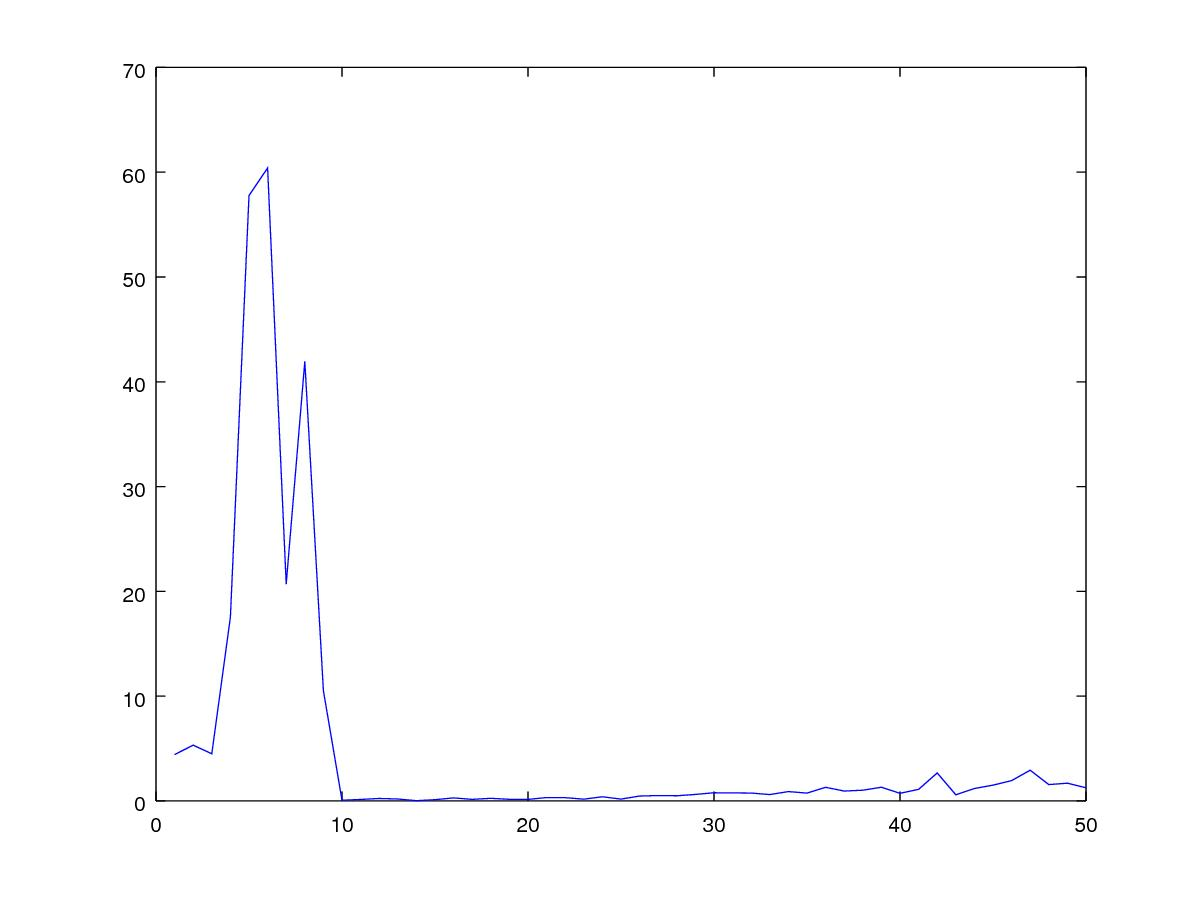
\includegraphics[width=90mm]{graph.jpg}
\caption{Mean Prediction Error with respect to n \label{overflow}}
\end{figure}
We can see that the error reaches its lowest point at around $n \in [10, 20]$ and then slowly begins to increase again as n increases.
\end{flushleft}
\pagebreak
\subsection{Computing Coefficients h if Input and Output Values are Constant}
\begin{flushleft}
What would the vector of coefficients look like if every input and output value were a constant? Let a be a constant value and let \begin{math}x_{i}= y_{i} = a, \, i \in [0, \, N]\end{math}. The matrix representation of the system of linear equations \begin{math} Ah = y \end{math} can be represented as:
\vspace{2mm}
\[
\begin{bmatrix}
    a & \hdotsfor{2} & a \\
    \vdots & \empty & \empty & \vdots \\
    a & \hdotsfor{2} & a
\end{bmatrix}
\begin{bmatrix}
    h_{1} \\
    \vdots \\
    h_{n}
\end{bmatrix}
=
\begin{bmatrix}
    a \\
    \vdots \\
    a
\end{bmatrix}
\]
\break
The linear combination of an arbitrary y value can be written as follows:
\begin{math}ah_{1} + \cdots + ah_{n} = a\end{math}
\break From this it follows that\newline	
\begin{math}a(h_{1} + \cdots + h_{n})= a\end{math} \newline
\begin{math}h_{1} + \cdots + h_{n} = 1\end{math}.
\end{flushleft}
This shows that every vector of coefficient h whose components add up to 1 will represent a solution of the system. \newline
If we require that \begin{math} \forall i, j \in [1, n]: h_{i} = h_{j}\end{math}, we can write that \begin{math} \forall i \in [1, n]: h_{i} = \frac{1}{n}\end{math}
\vspace{0.5cm}
\begin{flushleft}
\section{Implementation in MATLAB/Octave}
\begin{flushleft}
This section lays out a well-commented MATLAB/Octave implementation of the movavg and prediction functions described in the problem statement in section 1. \pagebreak
\subsection{movavg}\mbox{}\\
% Implementation of movavg in MATLAB/Octave
\end{flushleft}
\begin{footnotesize}
\begin{verbatim}
function [h] = movavg(x, y, n)

  % initialize empty matrix A
  A = [];
  % Initialize empty matrix for storing the next column to add to matrix A.
  next_column = [];
  
  % Outer loop runs on [n - 1, 0].
  % (the quantities subtracted from current t)
  for sub = n - 1 : -1 : 0
  
    % Inner loop runs on [n, N].
    % (quantities representing the current t)
    for k = n : size(x)(2)
      % Add appropriate x value to next_column vector.
      next_column = [next_column; x(k - sub)];
    end
    % Put constructed column into the A matrix.
    A = [A, next_column];
    % Prepare the next_column vector for next iteration (empty it).
    next_column = [];   
  end
  % Before solving, vector y must be truncated as
  % we can only predict values y(t) where t >= n - 1.
  y = y(:, n:end);
  
  % Make y a column vector and solve system of equations for h.
  h = A\y';
  h = h';
endfunction
\end{verbatim}
\end{footnotesize}
\end{flushleft}
\pagebreak

\subsection{prediction}
% Implementation of movavg in MATLAB/Octave
\begin{footnotesize}
\begin{verbatim}
function [h] = movavg(x, y, n)

  % initialize empty matrix A
  A = [];
  % Initialize empty matrix for storing the next column to add to matrix A.
  next_column = [];
  
  % Outer loop runs on [n - 1, 0].
  % (the quantities subtracted from current t)
  for sub = n - 1 : -1 : 0
  
    % Inner loop runs on [n, N].
    % (quantities representing the current t)
    for k = n : size(x)(2)
      % Add appropriate x value to next_column vector.
      next_column = [next_column; x(k - sub)];
    end
    % Put constructed column into the A matrix.
    A = [A, next_column];
    % Prepare the next_column vector for next iteration (empty it).
    next_column = [];   
  end
  % Before solving, vector y must be truncated as
  % we can only predict values y(t) where t >= n - 1.
  y = y(:, n:end);
  
  % Make y a column vector and solve system of equations for h.
  h = A\y';
  h = h';
endfunction
\end{verbatim}
\end{footnotesize}

\end{document}